\chapter{Weitere Prinzipien}

\section{Analyse GRASP: Geringe Kopplung}
\subsection*{Positiv-Beispiel}
\vspace{0.5cm}
\begin{figure}[H]
    \centering
    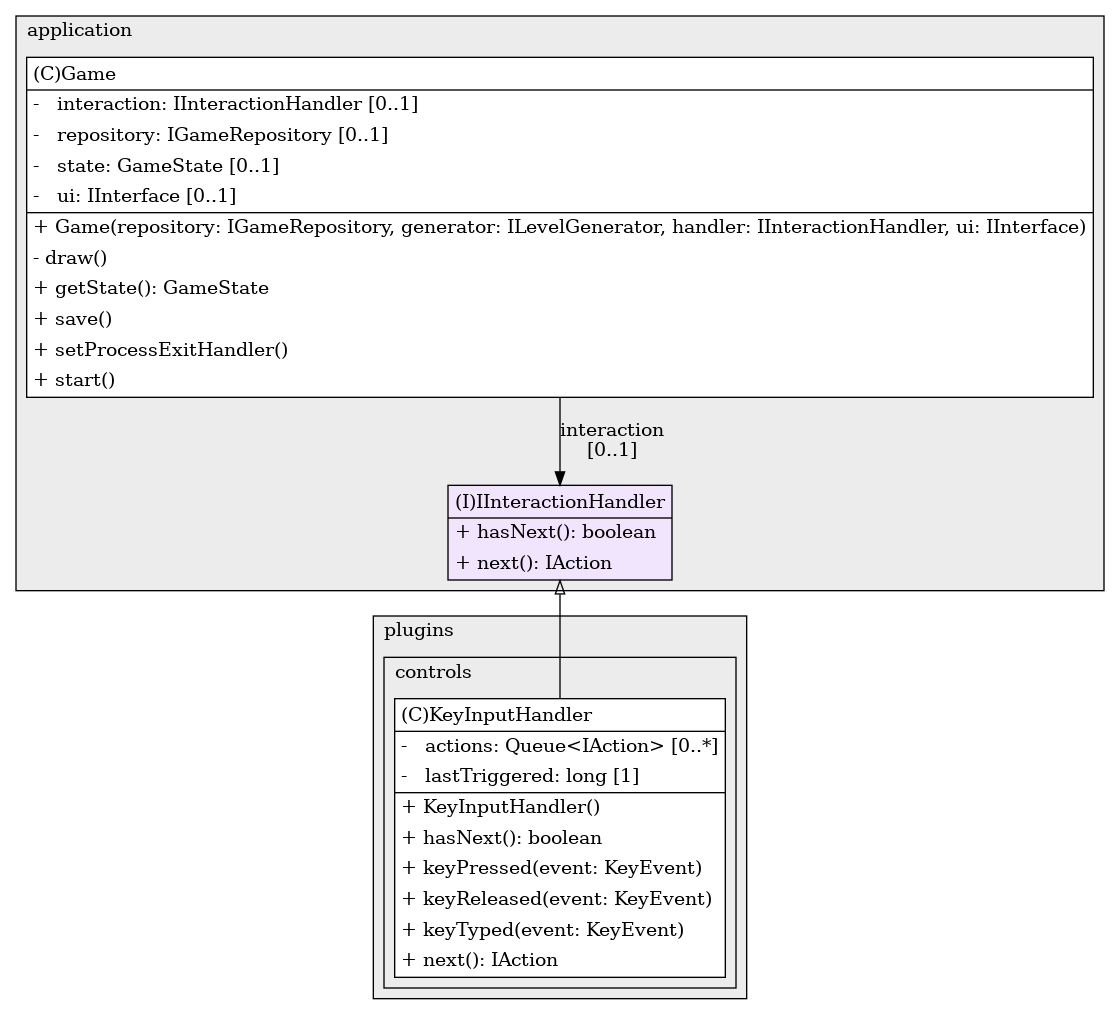
\includegraphics[width=1\linewidth]{Bilder/Visualisierung/IInteractionHandler_structure.png}
    \caption{Analyse GRASP: Geringe Kopplung / Positiv}
\end{figure}

\subsection*{Negativ-Beispiel}
\vspace{0.5cm}
\begin{figure}[H]
    \centering
    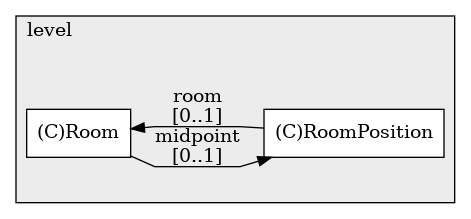
\includegraphics[width=1\linewidth]{Bilder/Visualisierung/RoomPositionNoInterface_structure.png}
    \caption{Analyse GRASP: Geringe Kopplung / Negativ}
\end{figure}

\iffalse
Um die beiden Klassen RoomPosition und Room besser zu entkoppeln, können wir die direkte Abhängigkeit der RoomPosition von der konkreten Room-Implementierung lösen und stattdessen eine abstrakte Schnittstelle oder eine abstrakte Basisklasse einführen. Dadurch wird die Abhängigkeit lockerer und die Klassen können unabhängig voneinander entwickelt, getestet und gewartet werden.

Hier ist ein Beispiel, wie die Klassen entkoppelt werden könnten:

java
Copy code
public interface Room {
    boolean contains(Position position);
    boolean isBlockedByEnemy(Position position);
}

public class ConcreteRoom implements Room {
    // Implementierung der Methoden für den konkreten Raum
    // ...
}

public class RoomPosition extends Position implements IVectorizable {
    private final Room room;

    public RoomPosition(int x, int y, Room room) {
        super(x, y);
        this.room = room;
    }

    public Room getRoom() {
        return this.room;
    }

    public boolean isInside() {
        return this.room.contains(this);
    }

    public boolean isBlockedByEnemy() {
        return this.room.isBlockedByEnemy(this);
    }

    // Restliche Methoden und Implementierung der Klasse
    // ...
}
In diesem Beispiel haben wir die Schnittstelle Room eingeführt, die die benötigten Methoden definiert, die die RoomPosition verwenden möchte. Die konkrete Implementierung ConcreteRoom implementiert diese Schnittstelle und enthält die spezifische Logik für den Raum.

Durch die Verwendung der Schnittstelle Room anstelle der konkreten Room-Klasse wird die Abhängigkeit in der RoomPosition gelockert. Jetzt kann die RoomPosition mit jeder Klasse arbeiten, die die Room-Schnittstelle implementiert, unabhängig von ihrer konkreten Implementierung.

Dies ermöglicht es uns, verschiedene Arten von Räumen zu erstellen und auszutauschen, ohne dass Änderungen an der RoomPosition erforderlich sind. Außerdem erleichtert es das Testen der RoomPosition, da wir Mock-Implementierungen der Room-Schnittstelle verwenden können, um isolierte Tests durchzuführen.

Die Entkopplung der Klassen erhöht die Flexibilität, Wartbarkeit und Testbarkeit des Codes und fördert eine bessere Modulbildung und Wiederverwendbarkeit der Komponenten.

\fi

\section{Analyse GRASP: Hohe Kohäsion}

\iffalse
Die gegebene Klasse "Buffer" erfüllt das Kriterium der hohen Kohäsion, da sie eine klare und spezifische Aufgabe erfüllt, nämlich die Verwaltung eines Puffers für die Darstellung von Zeichen und Farben. Hier sind einige Gründe, warum sie hohe Kohäsion aufweist:

Zusammengehörigkeit: Die Methoden und Eigenschaften der Klasse dienen alle dem Zweck der Pufferverwaltung. Sie ermöglichen das Setzen von Zeichen und Farben, das Hinzufügen von Inhalten, das Erzeugen von speziellen Puffern (z. B. mit Rahmen) und die Darstellung des Puffers.

Klare Verantwortlichkeiten: Die Klasse konzentriert sich ausschließlich auf die Pufferverwaltung und enthält keine Funktionalitäten, die nicht damit verbunden sind. Sie bietet Methoden zum Setzen von Zeichen, Farben, zum Schreiben von Inhalten, zum Erzeugen spezieller Puffer und zur Darstellung des Puffers.

Geringe Abhängigkeit von externen Komponenten: Die Klasse hat keine Abhängigkeiten von anderen Klassen oder externen Ressourcen. Sie enthält alle erforderlichen Methoden und Datenstrukturen, um die Pufferverwaltung durchzuführen.

Einfache Wiederverwendbarkeit: Der Buffer kann in verschiedenen Anwendungen oder Modulen wiederverwendet werden, in denen eine Pufferverwaltung erforderlich ist. Die Klasse ist gut isoliert und unabhängig von anderen Teilen des Systems.

Insgesamt erfüllt die Klasse "Buffer" das Prinzip der hohen Kohäsion, indem sie eine klare und spezifische Aufgabe erfüllt und ihre Methoden und Eigenschaften darauf ausgerichtet sind. Dies erleichtert die Lesbarkeit, Wartbarkeit und Wiederverwendbarkeit des Codes.
\fi

\section{Don't Repeat Yourself (DRY)}